\chapter{Event Selection}

\label{ch:selection}

The \acp{LLP} targeted by this search differ in their interactions with the detector from other, \ac{SM} particles primarily because of their large mass. 
That large mass results in a low $\beta$ when produced at the energies available at the \ac{LHC}, and such slow-moving particles heavily ionize in detector material when charged. 
Each layer of the pixel detector provides a measurement of that ionization, through \ac{ToT}, as discussed in Section~\ref{sec:pixel}. 
The ionization in the pixel detector, quantified in terms of \dedx, provides the major focus for this search technique, both because of its discriminating power and also because of the large range of lifetimes where it can be used.

The \dedx variable needs to be augmented with a few additional selection requirements to form a complete search. 
Ionization is not currently available in any form during triggering, so this search instead relies on \met to trigger the events out of necessity. 
Although triggering on \met is not particularly efficient, \met is often large for many production mechanisms of \acp{LLP}, as discussed in Section~\ref{sec:characteristics}.

Ionization is most effective in rejecting backgrounds for well-measured, high-momentum tracks, so some basic requirements on quality and kinematics are placed on the particles considered in this search. 
In particular a newly introduced tracking variable (referred to as \Nss and defined in detail in Section~\ref{sec:track_requirements}) is very effective in removing highly-ionizing backgrounds caused by overlapping tracks. 
A few additional requirements are placed on the tracks considered for \ac{LLP} candidates that increase background rejection by targeting specific types of \ac{SM} particles (Section~\ref{sec:sm_rejection}). 
These techniques provide a significant analysis improvement over previous iterations of ionization-based searches on ATLAS by providing additional background rejection with minimal loss in signal efficiency. 

The ionization measurement with the Pixel detector can be calibrated to provide an estimator of $\beta\gamma$. That estimate, together with the momentum measurement provided by tracking, can be used to reconstruct a mass for each track which traverses the pixel detector. 
That mass variable will be peaked at the \ac{LLP} mass for any signal, and provides an additional tool to search for an excess.
In addition to an explicit requirement on ionization, this search constructs a mass-window for each targeted mass range in order to evaluate any excess of events and to set limits. 
Construction, calibration, and requirements for the mass variable are discussed in Section~\ref{sec:mass_requirement}.

The strategy discussed here is optimized for lifetimes of $O(1)$ - $O(10)$ ns. 
Pixel ionization is especially useful in this regime as particles only need to propagate through the first seven layers of the inner detector, about 37 cm from the beam axis. 
The search is still competitive with other searches for \acp{LLP} at longer lifetimes, because the primary discriminating variables are still applicable even for particles that do not decay within the detector. 
Although the basic strategy remains the same for all lifetimes, two signal regions are defined to optimize separately for intermediate and long lifetime particles (Section~\ref{sec:sm_rejection}). 


% --------------------------------------------------------------------------------

\section{Trigger}

Triggering remains one of the primary difficulties in defining an event selection with high signal efficiency in a search for \acp{LLP}. 
There are no triggers available in the current ATLAS system that can fire directly from a high momentum track with large ionization (Section~\ref{sec:trigger}). 
Although in some configurations a charged \ac{LLP} can fire muon triggers, this requirement introduces significant model dependence on both the allowed lifetimes and the interactions in the calorimeter.

For a search targetting particles which may decay prior to reaching the muon system, the most efficient available trigger is based on missing energy.
As discussed in Section~\ref{sec:characteristics}, signal events can produce \met by two primary mechanisms.
The decays of \rhadrons to neutralinos can produce missing energy when the neutralinos go undetected in the detector.
\acp{LLP} which do not decay before the calorimeters also can produce missing energy because they do not deposit much of their energy in the calorimeter. 
Either case to some extent relies on kinematic degrees of freedoms to produced missing energy, as the pair-produced \acp{LLP} tend to balance each other in the transverse plain.
That balance results in a relatively low efficiency for long-lifetime particles, roughly 40\%, and efficiencies between 65\% and 95\% for shorter lifetimes depending on both the mass and the lifetime, as seen in Figure~\ref{fig:trigger_efficiency}. 

\begin{figure}[h]
\centering
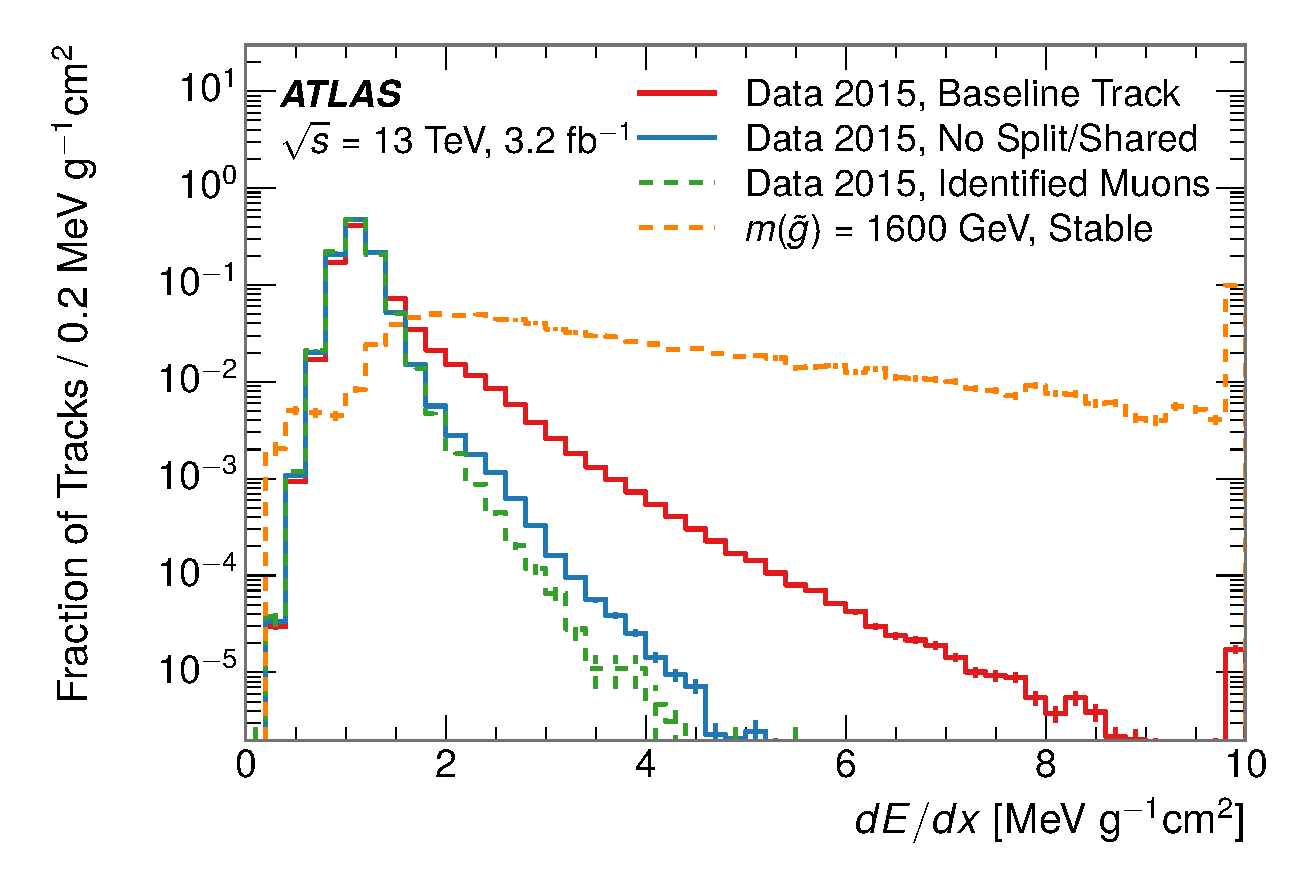
\includegraphics[draft, width=.68\textwidth]{figures/trigger_efficiency.pdf}
\caption{The trigger efficiency of the \met trigger as a function of mass and lifetime.}
\label{fig:trigger_efficiency}
\end{figure}

% ----------------------------------------

\section{Kinematics and Isolation}
\label{sec:track_requirements}

After the trigger requirement, each event is required to have a primary vertex reconstructed from at least two well-measured tracks in the inner detector, each with $\pt > 400$ MeV. 
If more than one such vertex exists, the primary vertex is taken to be the one with the largest summed track momentum for all tracks associated to that vertex. 
The offline reconstructed \met is required to be above 130 GeV to additionally reject \SM backgrounds.
The transverse missing energy is calculated using fully reconstructed and calibrated offline objects, as described in Section~\ref{sec:missing_energy}. 
In particular the \met definition in this selection uses jets reconstructed with the anti-$k_t$ algorithm with radius $R = 0.4$ from clusters of energy in the calorimeter (Section~\ref{sec:jets}) and with $p_T > 20 \GeV$, as well as reconstructed muons, electrons, and tracks not identified as another object type.
The \met distributions are shown for data and a few simulated signals in Figure~\ref{fig:nm1_met}, after the trigger requirement.
The cut placed at 130 GeV is 95\% efficient for metastable and 90\% efficient for stable particles, because of the missing energy generating mechanisms discussed previously.

\begin{figure}[h]
\centering
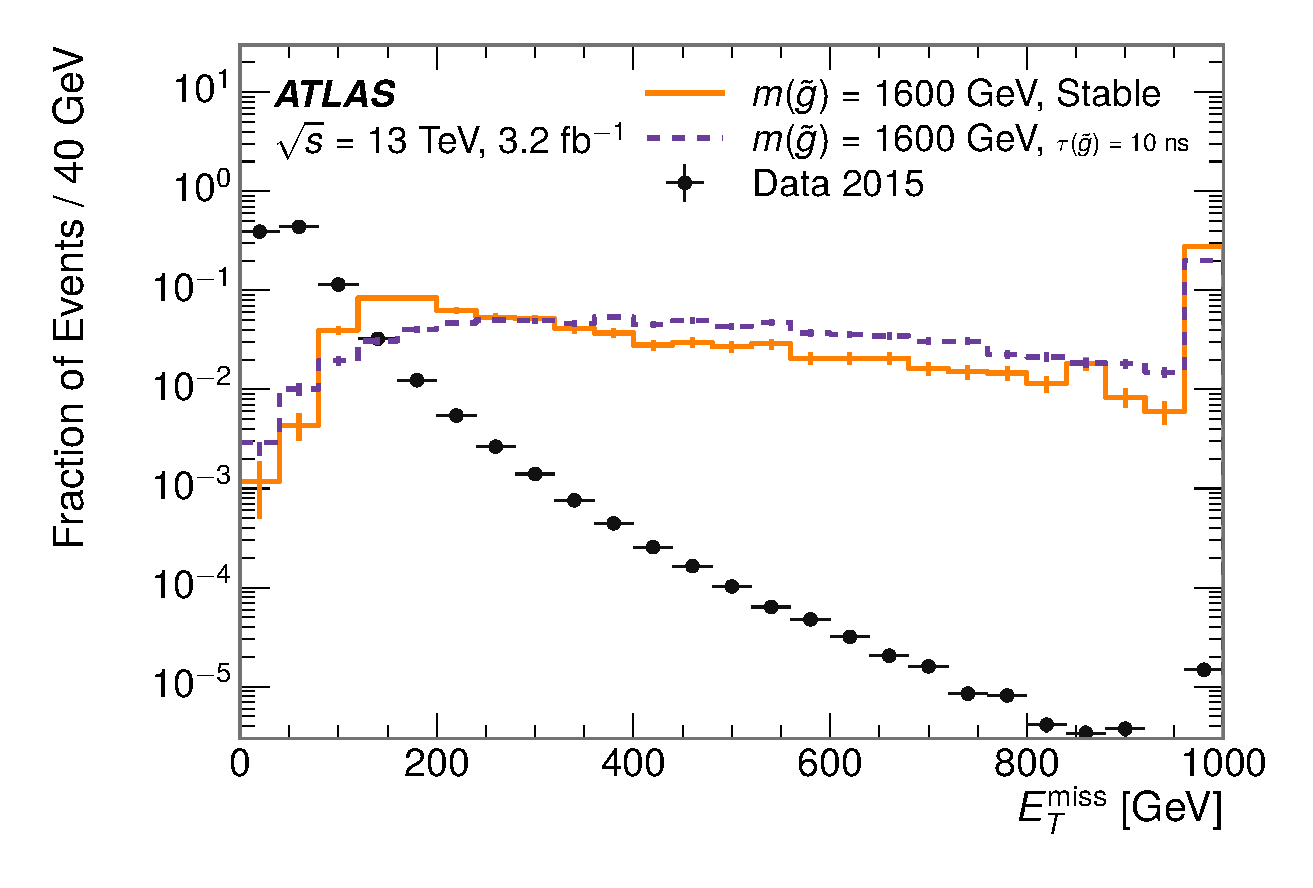
\includegraphics[width=0.68\textwidth]{figures/selection_met_nm1_log.pdf}
\caption{The distribution of \met for data and simulated signal events, after the trigger requirement.}
\label{fig:nm1_met}
\end{figure}

Potential signal events are then required to have at least one candidate \ac{LLP} track.
Although the \acp{LLP} are produced in pairs, many models do not consistently yield two charged particles.
For example, in the \rhadron model highlighted here, only 20\% of events have two charged \rhadrons while 47\% of events have just one.

For a track to be selected as a candidate, it must have $p_T > 50$ \GeV and pass basic quality requirements. 
In particular, it must have at least seven clusters in the silicon detector layers in the inner detector to ensure an accurate measurement of momentum including one cluster in the innermost layer if it is expected geometrically. 
The track must additionally be associated to the primary vertex.


\begin{figure}[h]
\centering
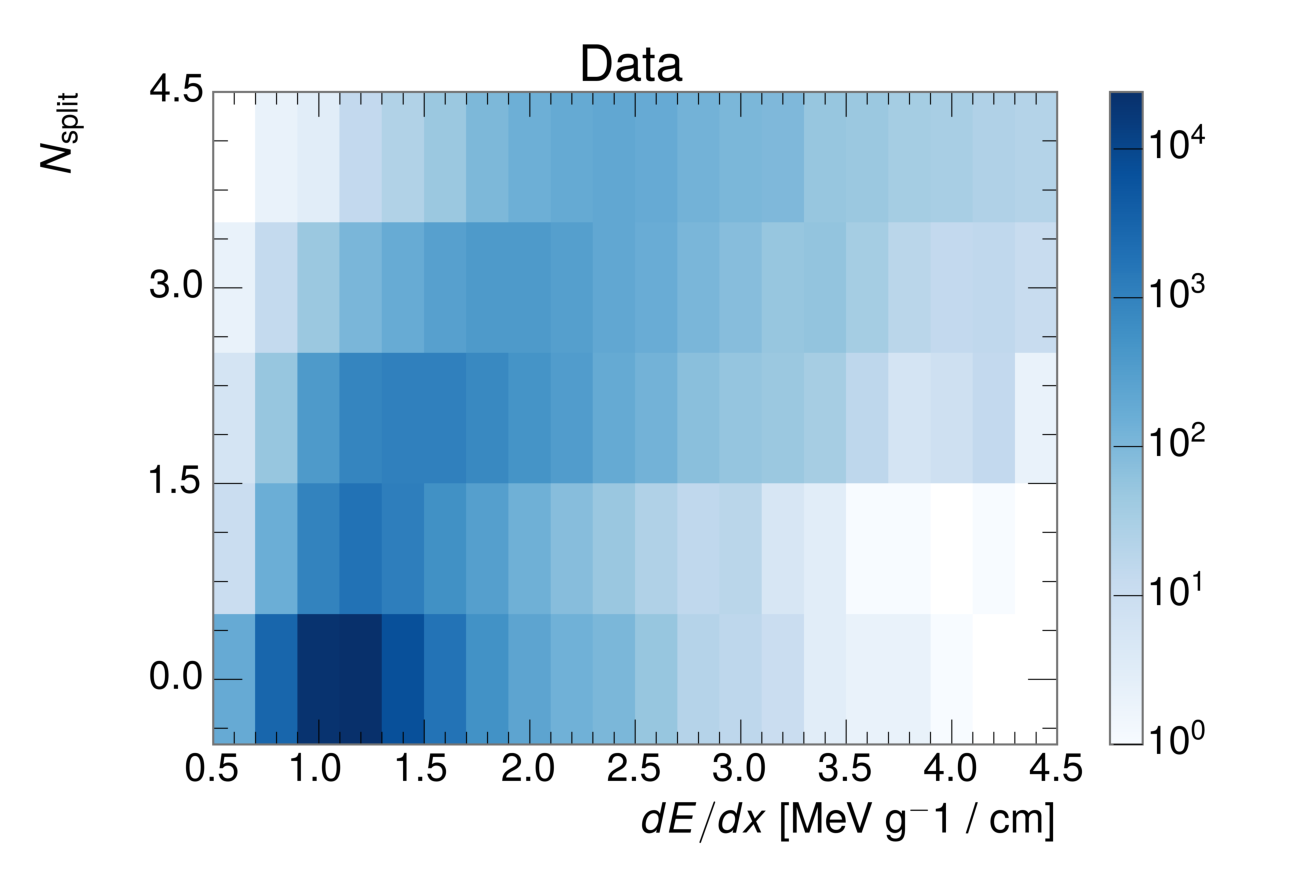
\includegraphics[width=0.68\textwidth]{figures/dedx_nsplit_data.pdf}
\caption{The dependence of \dedx on $N_{\mathrm{split}}$ in data after basic track hit requirements have been applied.}
\label{fig:dedx_nsplit}
\end{figure}

\begin{figure}[h]
\centering
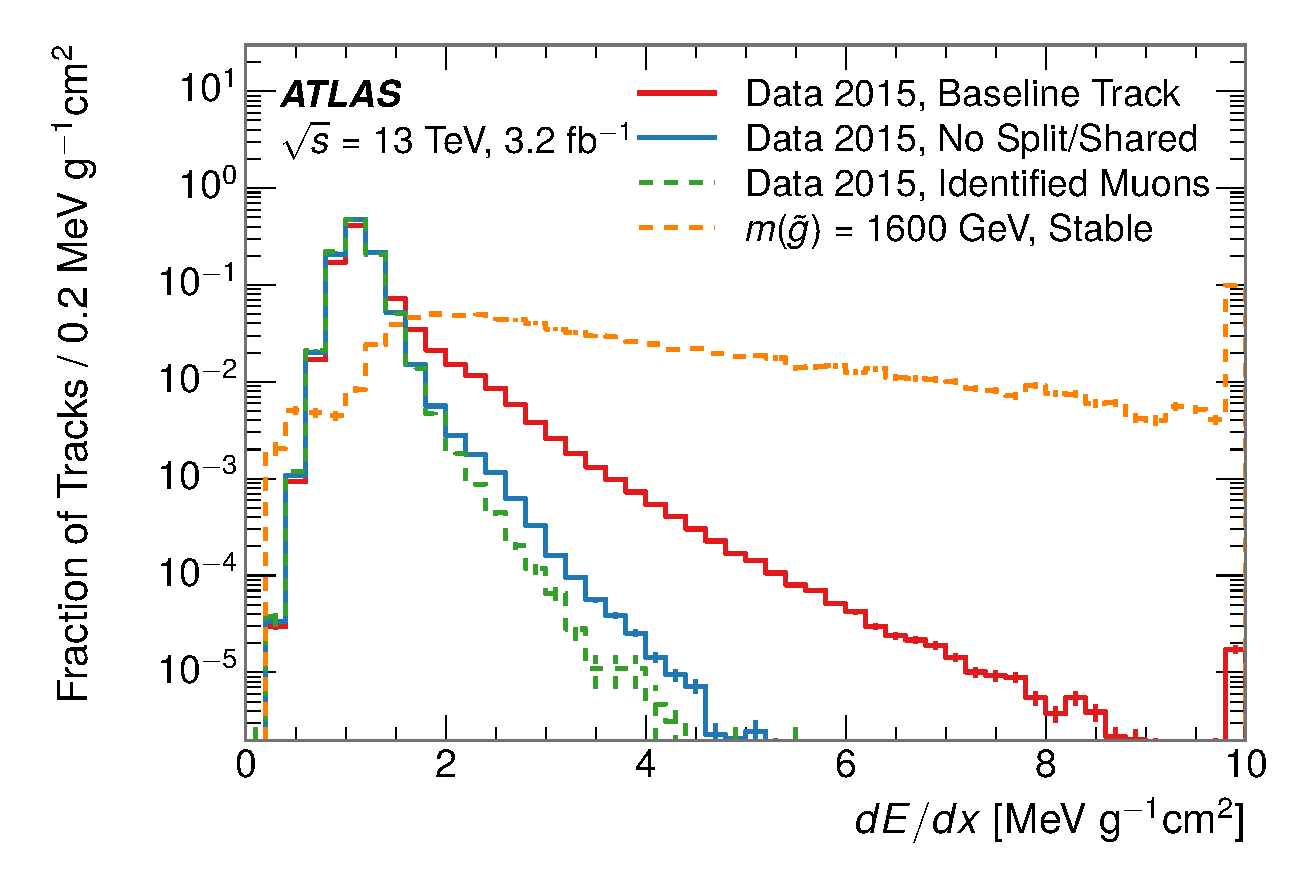
\includegraphics[width=0.68\textwidth]{figures/dedx_isolation.pdf}
\caption{The distribution of \dedx with various selections applied in data and simulated signal events.}
\label{fig:dedx_nsplit}
\end{figure}

\begin{figure}[h]
\centering
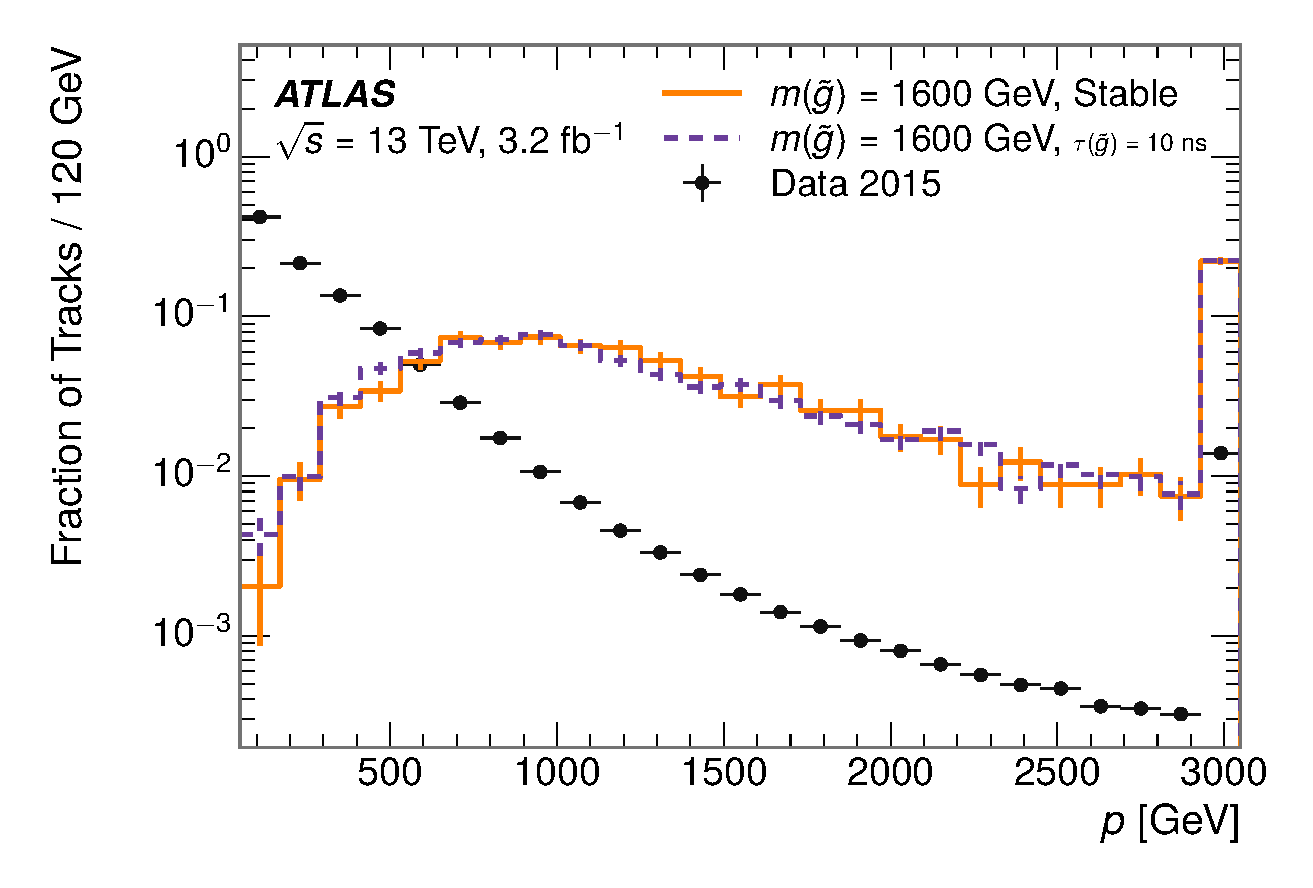
\includegraphics[width=0.68\textwidth]{figures/selection_p_nm1.pdf}
\caption{The distribution of track momentum for data and simulated signal events, after previous selection requirements have been applied.}
\label{fig:nm1_p}
\end{figure}

% ----------------------------------------

\section{Standard Model Rejection}
\label{sec:sm_rejection}



\begin{figure}[h]
\centering
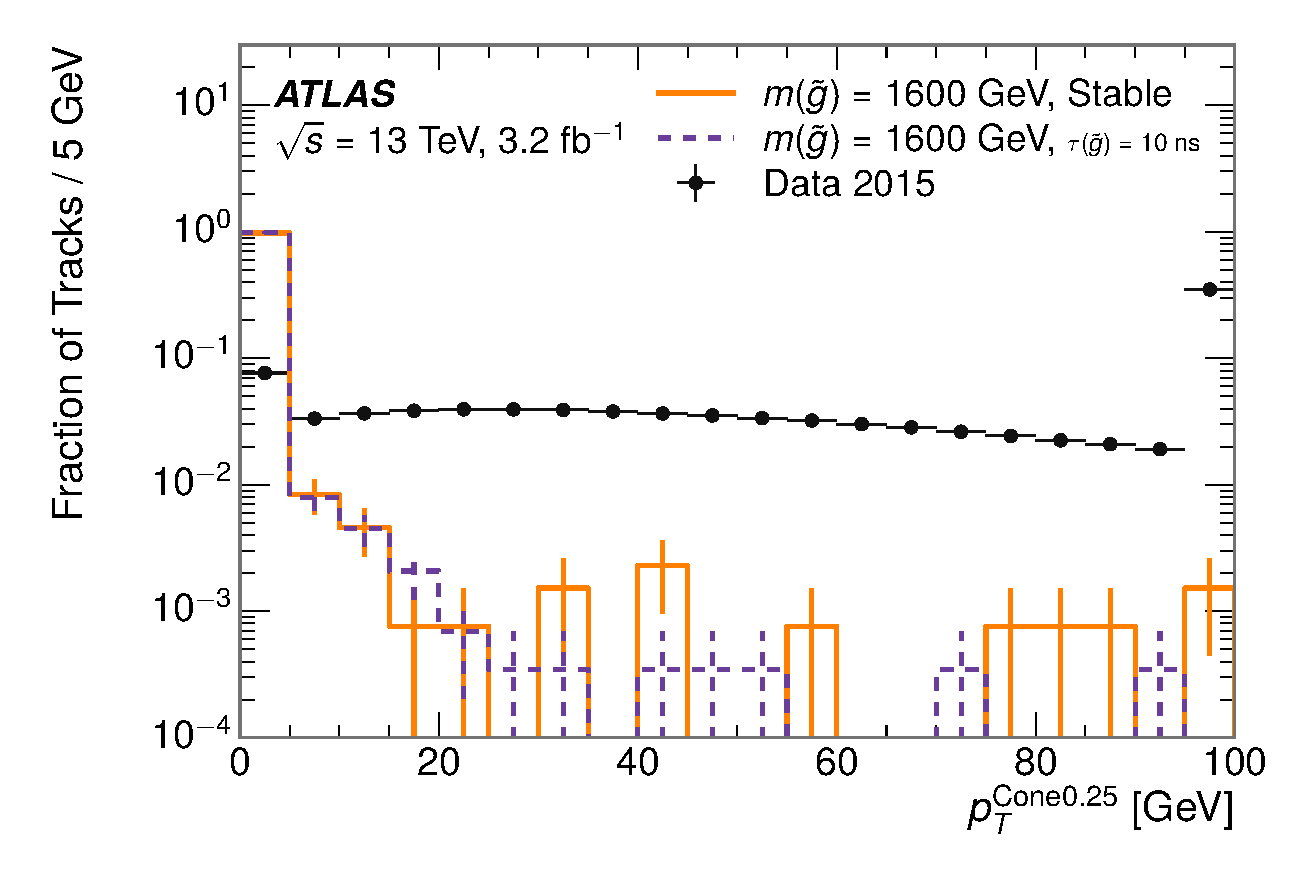
\includegraphics[width=0.68\textwidth]{figures/selection_isopt_nm1.pdf}
\caption{The distribution of summed tracked momentum within a cone of $\Delta R < 0.2$ around the candidate track for data and simulated signal events, after previous selection requirements have been applied.}
\label{fig:nm1_isopt}
\end{figure}

\begin{figure}[htb]
\centering
\subfloat[]{
  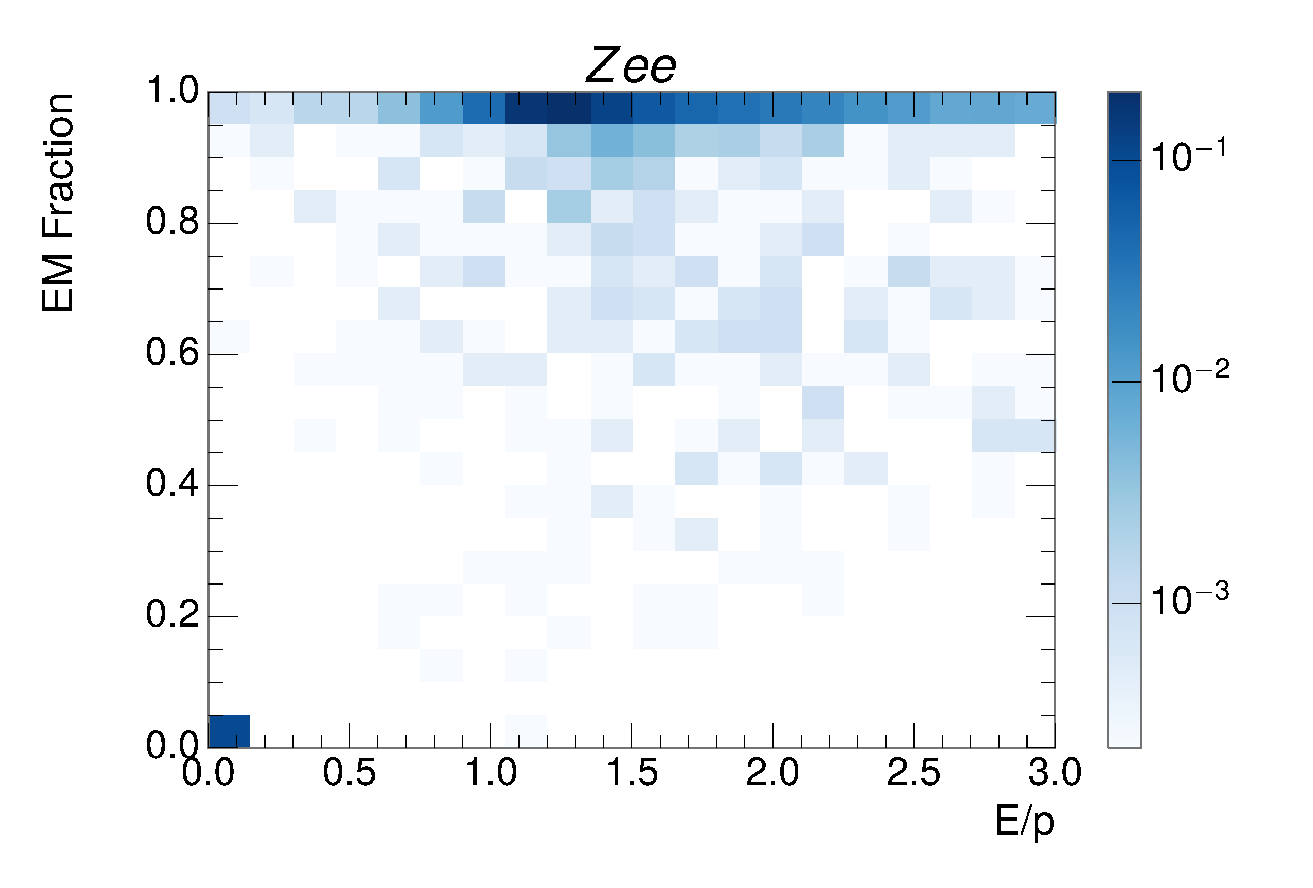
\includegraphics[width=0.48\textwidth]{figures/zee_eoverp_emfrac.pdf}
}
\subfloat[]{
  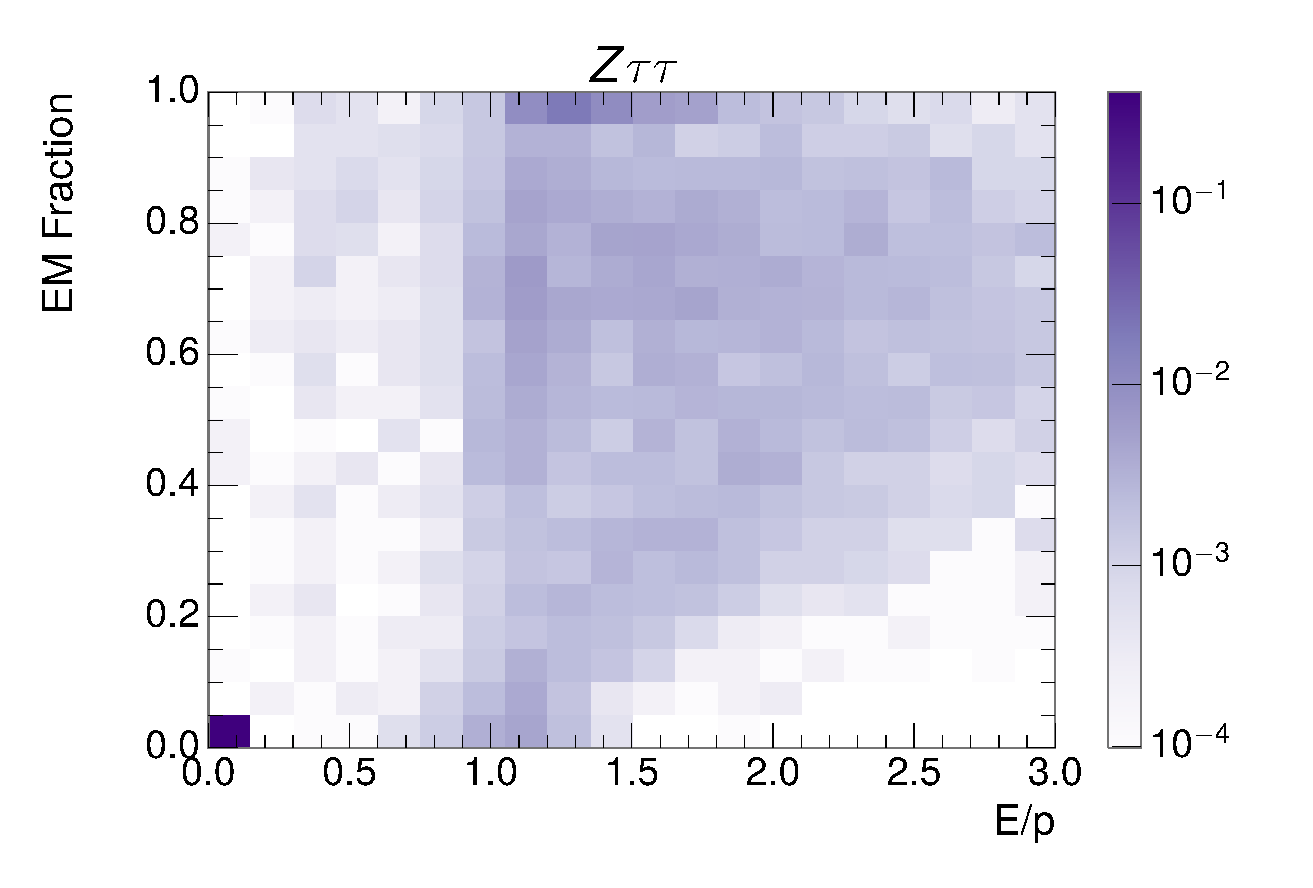
\includegraphics[width=0.48\textwidth]{figures/ztautau_eoverp_emfrac.pdf}
}\\
\subfloat[]{
  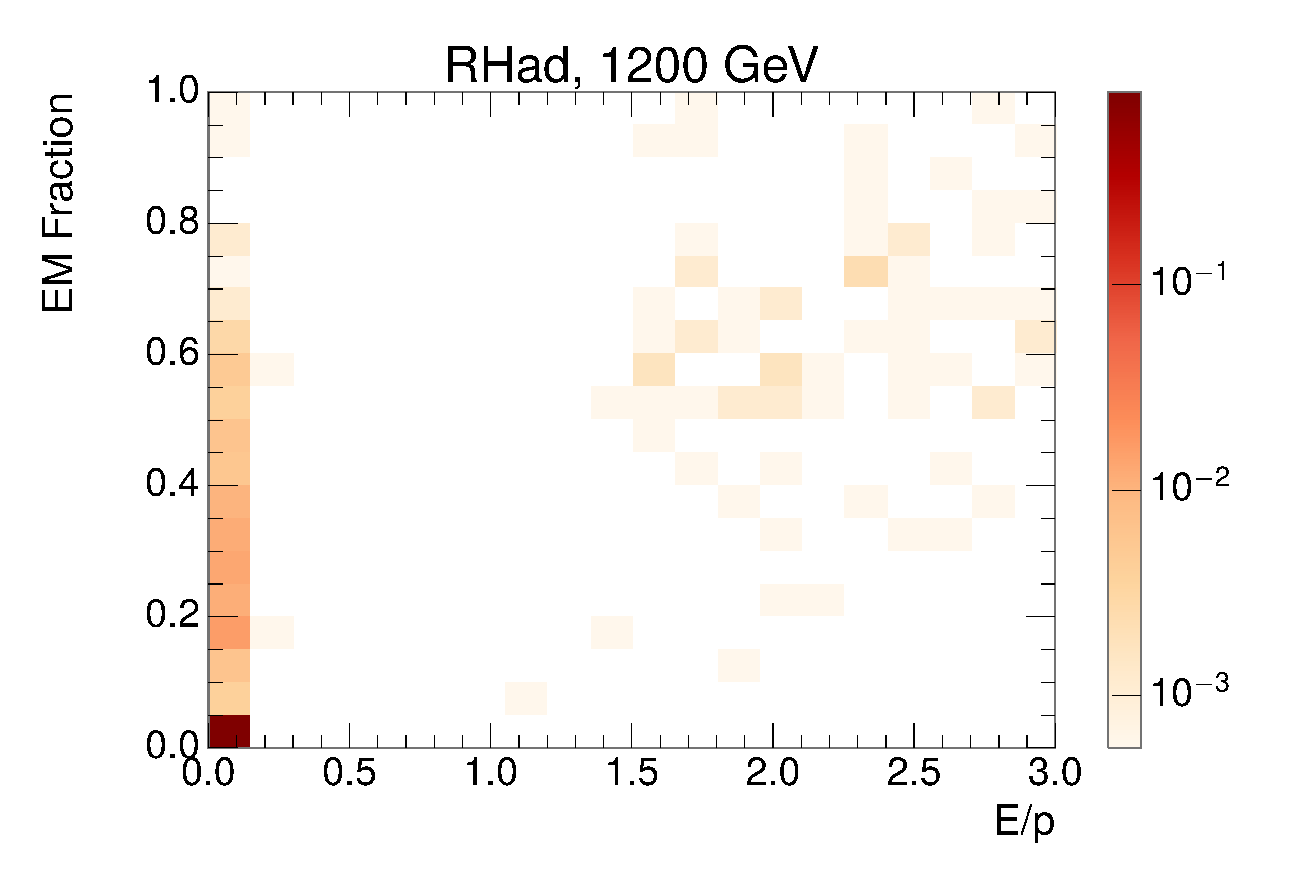
\includegraphics[width=0.48\textwidth]{figures/rhad_eoverp_emfrac.pdf}
}
\caption{The normalized, two-dimensional distribution of $E/p$ and EM fraction for simulated (a) $Z\rightarrow ee$, (b) $Z\rightarrow \tau\tau$ and (c) 1200 GeV R-Hadron events.}
\label{fig:nm1_isopt}
\end{figure}


% ----------------------------------------

\section{Ionization}

\subsection{dE/dx Calibration}

\subsection{Mass Estimation}
\label{sec:mass_requirement}
% ----------------------------------------
